\documentclass{standalone}
\usepackage{tikz}
\usepackage{verbatim}
\usetikzlibrary{positioning}
\begin{document}
\pagestyle{empty}
  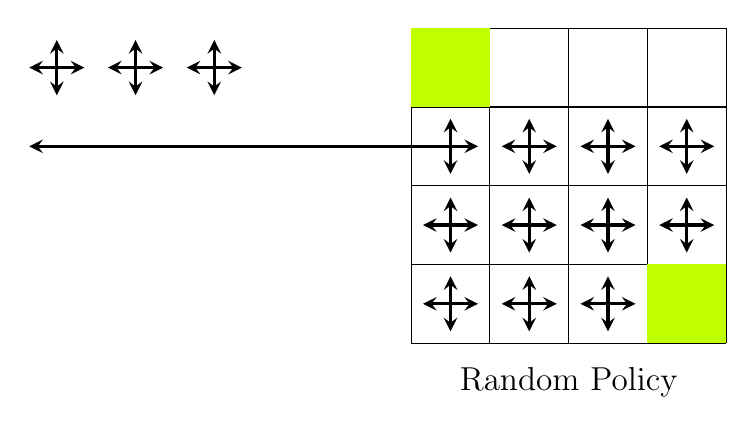
\begin{tikzpicture}

    \draw[step=1.0,black,thin] (5,0) grid (9, 4);
    \fill[lime] (5, 3) rectangle (6,4);
    \fill[lime] (8, 0) rectangle (9,1);
    % Top row.
    \draw[stealth-stealth, line width=0.4mm] (0.15, 3.5) -- (0.85, 3.5);
    \draw[stealth-stealth, line width=0.4mm] (0.5, 3.15) -- (0.5, 3.85);
    \draw[stealth-stealth, line width=0.4mm] (1.15, 3.5) -- (1.85, 3.5);
    \draw[stealth-stealth, line width=0.4mm] (1.5, 3.15) -- (1.5, 3.85);
    \draw[stealth-stealth, line width=0.4mm] (2.15, 3.5) -- (2.85, 3.5);
    \draw[stealth-stealth, line width=0.4mm] (2.5, 3.15) -- (2.5, 3.85);
    % Second from top row.
     \draw[stealth-stealth, line width=0.4mm] (0.15, 2.5) -- (5.85, 2.5);
    \draw[stealth-stealth, line width=0.4mm] (5.5, 2.15) -- (5.5, 2.85);
    \draw[stealth-stealth, line width=0.4mm] (6.15, 2.5) -- (6.85, 2.5);
    \draw[stealth-stealth, line width=0.4mm] (6.5, 2.15) -- (6.5, 2.85);
    \draw[stealth-stealth, line width=0.4mm] (7.15, 2.5) -- (7.85, 2.5);
    \draw[stealth-stealth, line width=0.4mm] (7.5, 2.15) -- (7.5, 2.85);
    \draw[stealth-stealth, line width=0.4mm] (8.15, 2.5) -- (8.85, 2.5);
    \draw[stealth-stealth, line width=0.4mm] (8.5, 2.15) -- (8.5, 2.85);
    % Second from bottom row.
    \draw[stealth-stealth, line width=0.4mm] (5.15, 1.5) -- (5.85, 1.5);
    \draw[stealth-stealth, line width=0.4mm] (5.5, 1.15) -- (5.5, 1.85);
    \draw[stealth-stealth, line width=0.4mm] (6.15, 1.5) -- (6.85, 1.5);
    \draw[stealth-stealth, line width=0.4mm] (6.5, 1.15) -- (6.5, 1.85);
    \draw[stealth-stealth, line width=0.4mm] (7.15, 1.5) -- (7.85, 1.5);
    \draw[stealth-stealth, line width=0.4mm] (7.5, 1.15) -- (7.5, 1.85);
    \draw[stealth-stealth, line width=0.4mm] (8.15, 1.5) -- (8.85, 1.5);
    \draw[stealth-stealth, line width=0.4mm] (8.5, 1.15) -- (8.5, 1.85);
    % Bottom row.
    \draw[stealth-stealth, line width=0.4mm] (6.15, 0.5) -- (6.85, 0.5);
    \draw[stealth-stealth, line width=0.4mm] (6.5, 0.15) -- (6.5, 0.85);
    \draw[stealth-stealth, line width=0.4mm] (7.15, 0.5) -- (7.85, 0.5);
    \draw[stealth-stealth, line width=0.4mm] (7.5, 0.15) -- (7.5, 0.85);
    \draw[stealth-stealth, line width=0.4mm] (5.15, 0.5) -- (5.85, 0.5);
    \draw[stealth-stealth, line width=0.4mm] (5.5, 0.15) -- (5.5, 0.85);
    \node at (7, -0.5) {\large Random Policy};

  \end{tikzpicture}
\end{document}